\documentclass[a4paper]{extarticle}
\usepackage[utf8]{inputenc}
\usepackage{hyperref}
\usepackage{geometry}
\usepackage{fancyhdr}
\usepackage{graphicx} % libreria per le immagini
\usepackage{amssymb} %libreria per i simboli (ex. alfabeto reco)
\usepackage{algorithm2e} %libreria per scrivere pseudocodice
\usepackage{longtable}
\usepackage{caption}
\usepackage{lastpage}
\usepackage{adjustbox}
\usepackage{ellipsis}
\usepackage{listings}
\usepackage{xcolor}
\usepackage{mathtools}

\definecolor{backcolour}{rgb}{0.95,0.95,0.96}
\lstdefinestyle{mystyle}{
	backgroundcolor=\color{backcolour},
	numbers=left,
	numbersep=5pt,
}
\lstset{style=mystyle, escapeinside={(*}{*)}}

\setlength{\parindent}{0em}%indentazione paragrafo
\setlength{\parskip}{1em}%spazio tra paragrafi
\renewcommand{\baselinestretch}{1.3}%interlinea
\graphicspath{ {./} }
\geometry{
    a4paper,
    left=10mm,
    right=10mm,
    bottom=20mm
}


\hypersetup{
    colorlinks=true,
    linkcolor=blue,
    filecolor=blue,      
    urlcolor=blue,
    pdftitle={Overleaf Example},
    pdfpagemode=FullScreen
}

\pagestyle{fancy}
\fancyhf{}
\rhead{Federico Calò}
\lhead{Ingegneria della conoscenza}
\cfoot{  \thepage }


\title{Ingegneria della conoscenza}
\author{\href{http://www.federicocalo.dev}{Federico Calò} }
\date{}

\begin{document}
\maketitle
\newpage
\tableofcontents
\voffset -30pt

\newpage

\section*{Premessa}

Questo file è il risultante della rielaborazione delle slide del professore Nicola Fanizzi, dell'università Aldo Moro di Bari, relative al corso di Ingegneria della conoscenza. Le slide sono state integrate con diversi appunti. 

Questo file non sostituisce le slide che il professore distribuisce durante il suo corso, tanto meno il libro consigliato.

\newpage


\section{Introduzione}

Vi sono diverse definizioni di ingegneria della conoscenza, due possono essere:

"L'ingegneria della conoscenza studia la rappresentazione, l'acquisizione, il ragionamento, il processo decisionale e l'applicazione della conoscenza, inclusi i big data, l'apprendimento automatico, il data mining e la scoperta della conoscenza, il ragionamento incerto, la mappatura della conoscenza, la dimostrazione di teoremi della macchina, il sistema esperto, il gioco della macchina, la biblioteca digitale, eccetera..."

oppure

"L'ingegneria della conoscenza (KE) si riferisce a tutti gli aspetti tecnici, scientifici e sociali coinvolti nella costruzione, manutenzione e utilizzo di sistemi basati sulla conoscenza"

Tipicamente l'informazione è definita in termini di dati, conoscenza in termini di informazioni e sapienza in termini di conoscenza. Queste relazioni vengono espresse nella \textbf{piramide della conoscenza}.
\begin{center}
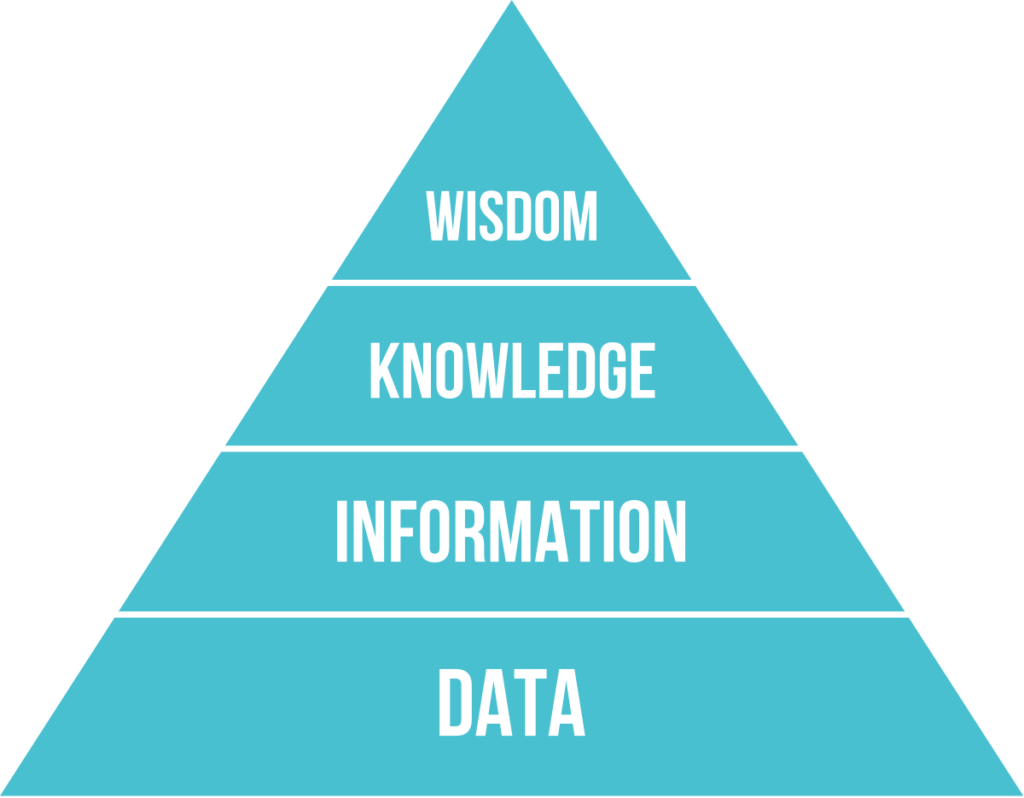
\includegraphics[scale=0.29]{PiramideDIKW}
\end{center}

I dati sono costituiti da simboli o segni ch reappresentano stimoli, segnali o fatti. Quando i dati assumono un significato o rappresentano uno scopo, generano l'informazione, la quale può essere strutturale o funzionale, simbolica o soggettiva. Successivamente quando si elabora, organizza e si applica l'informazione, si genera automaticamente la conoscenza.

L'\textbf{intelligenza artificiale} mira a studiare e comprendere i principi che rendono posiinile un comportamento intelligente in sistemi artificiali. L'ipotesi di base è che il ragionamento equivale in un certo senso alla computazione. La tesi di \textit{Church-Turing} definisce come \textbf{livello di astrazione} quel livello nel quale il ragionamento corrisponde alla manipolazione di simboli per spiegare le azioni/decisioni di un sistema tramite i suoi input.


\end{document}